\documentclass[border=8pt]{standalone}
\usepackage{tikz}
\usepackage{amsmath}
\usetikzlibrary{positioning,arrows.meta,fit,backgrounds,calc}
\begin{document}
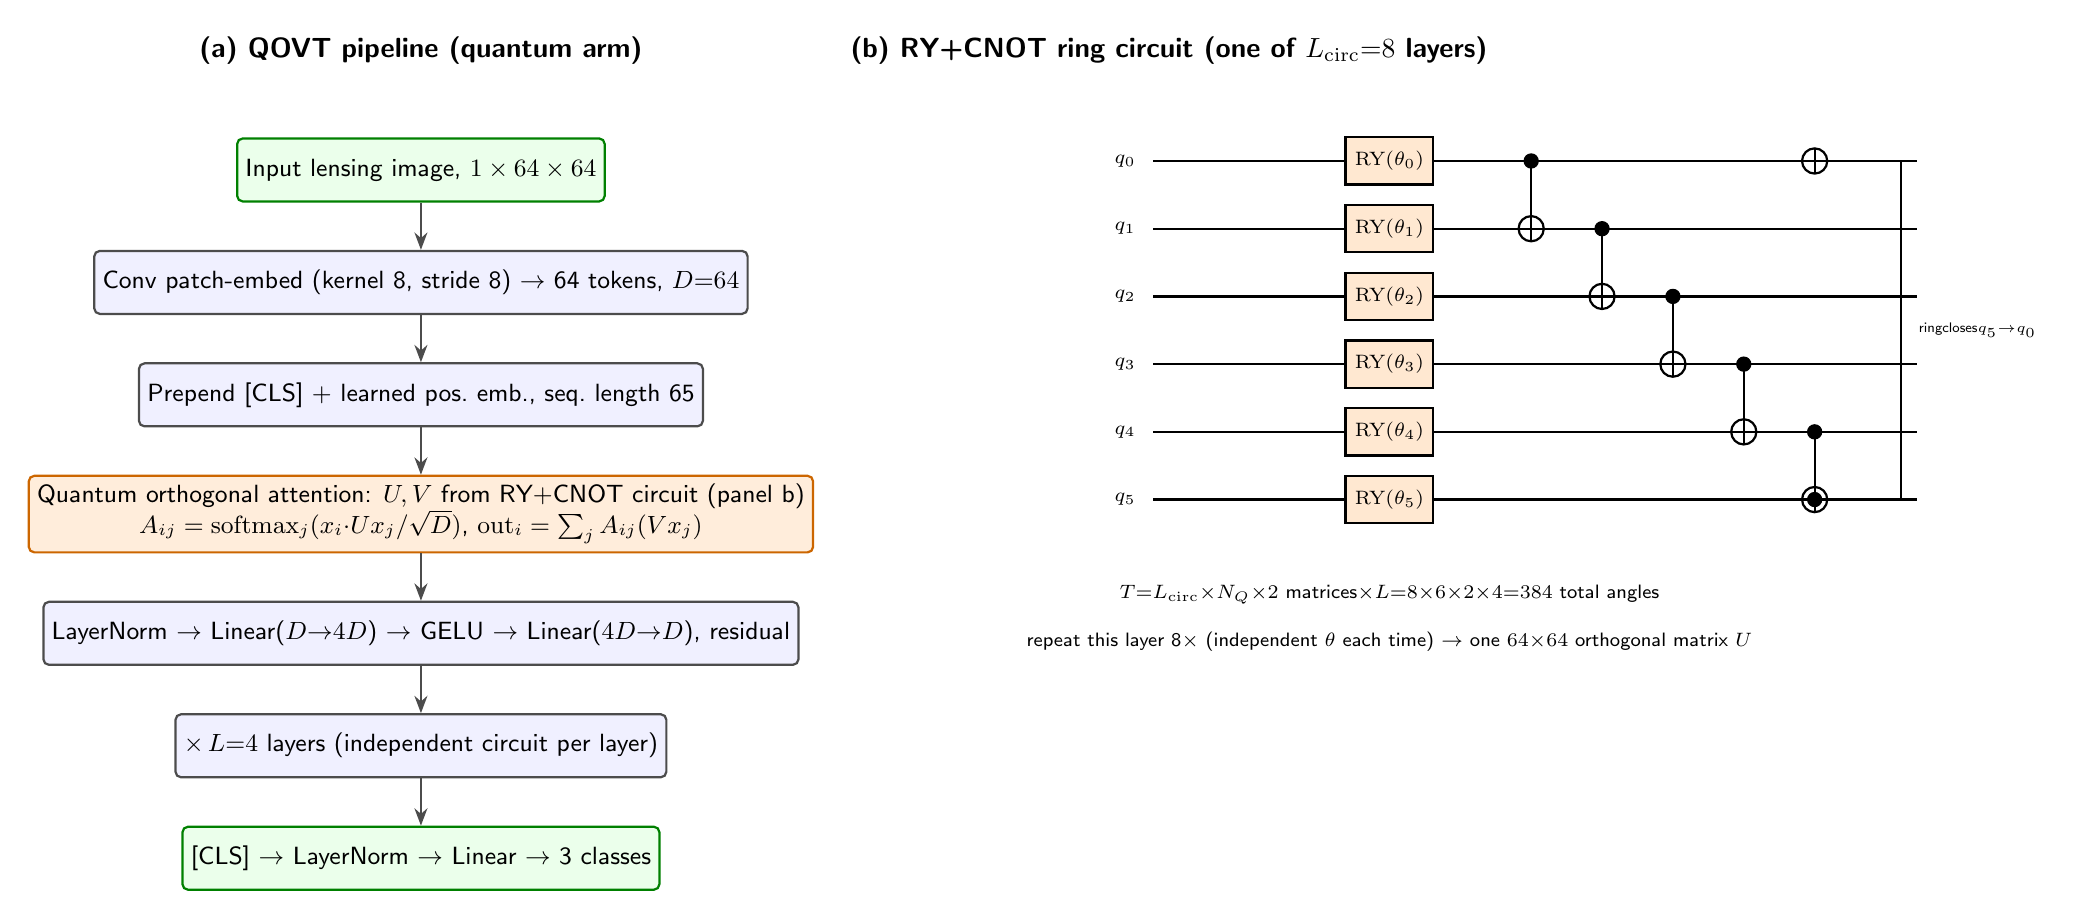
\begin{tikzpicture}[
  font=\sffamily\small,
  node distance=6mm,
  box/.style={rectangle,rounded corners=2pt,draw=black!70,thick,fill=blue!6,
              minimum height=8mm,minimum width=40mm,align=center,inner sep=3pt},
  io/.style={box,fill=green!8,draw=green!50!black},
  qbox/.style={box,fill=orange!14,draw=orange!80!black,minimum width=40mm},
  arr/.style={-{Stealth[length=2.2mm]},thick,black!70},
]

% ---------- Panel (a): quantum-only pipeline ----------
\node[font=\sffamily\bfseries\normalsize] (titleA) {(a) QOVT pipeline (quantum arm)};
\node[io,below=8mm of titleA] (img) {Input lensing image, $1\times64\times64$};
\node[box,below=of img] (patch) {Conv patch-embed (kernel 8, stride 8) $\to$ 64 tokens, $D{=}64$};
\node[box,below=of patch] (cls) {Prepend [CLS] + learned pos.\ emb., seq.\ length 65};
\node[qbox,below=of cls] (attn) {Quantum orthogonal attention: $U,V$ from RY+CNOT circuit (panel b)\\
  $A_{ij}=\mathrm{softmax}_j(x_i{\cdot}Ux_j/\sqrt{D})$, $\mathrm{out}_i=\sum_j A_{ij}(Vx_j)$};
\node[box,below=of attn] (mlp) {LayerNorm $\to$ Linear($D{\to}4D$) $\to$ GELU $\to$ Linear($4D{\to}D$), residual};
\node[box,below=of mlp,minimum width=52mm] (repeat) {$\times\,L{=}4$ layers (independent circuit per layer)};
\node[io,below=of repeat] (out) {[CLS] $\to$ LayerNorm $\to$ Linear $\to$ 3 classes};

\draw[arr] (img)--(patch);
\draw[arr] (patch)--(cls);
\draw[arr] (cls)--(attn);
\draw[arr] (attn)--(mlp);
\draw[arr] (mlp)--(repeat);
\draw[arr] (repeat)--(out);

% ---------- Panel (b): the RY+CNOT ring circuit, one layer ----------
% Convention: every macro below is a PLAIN NUMBER meaning millimetres;
% "mm" is appended explicitly at every point of use, never mixed bare.
\begin{scope}[xshift=95mm]
\node[font=\sffamily\bfseries\normalsize] (titleB) {(b) RY+CNOT ring circuit (one of $L_\mathrm{circ}{=}8$ layers)};

\pgfmathsetmacro{\qy}{8.6}   % vertical spacing between qubit lines, mm
\pgfmathsetmacro{\xstart}{0}
\pgfmathsetmacro{\xry}{28}
\pgfmathsetmacro{\xcnotstart}{46}
\pgfmathsetmacro{\xcnotstep}{9}
\pgfmathsetmacro{\ytop}{-14}  % vertical offset below the title, mm

\foreach \i in {0,...,5} {
  \pgfmathsetmacro{\y}{-\i*\qy+\ytop}
  \node[anchor=east,font=\sffamily\scriptsize] at (\xstart-3mm,\y mm) {$q_{\i}$};
  \pgfmathsetmacro{\xend}{\xcnotstart+5*\xcnotstep+4}
  \draw[thick] (\xstart-2mm,\y mm) -- (\xend mm,\y mm);
}

% RY gates on every qubit
\foreach \i in {0,...,5} {
  \pgfmathsetmacro{\y}{-\i*\qy+\ytop}
  \node[draw,fill=orange!18,thick,minimum width=9mm,minimum height=6mm,font=\scriptsize]
    at (\xry mm,\y mm) {RY$(\theta_{\i})$};
}

% CNOT ring: (0->1),(1->2),(2->3),(3->4),(4->5) nearest-neighbour
\foreach \c/\t/\k in {0/1/0, 1/2/1, 2/3/2, 3/4/3, 4/5/4} {
  \pgfmathsetmacro{\yc}{-\c*\qy+\ytop}
  \pgfmathsetmacro{\yt}{-\t*\qy+\ytop}
  \pgfmathsetmacro{\xg}{\xcnotstart+\k*\xcnotstep}
  \draw[thick] (\xg mm,\yc mm) -- (\xg mm,\yt mm);
  \filldraw (\xg mm,\yc mm) circle (0.9mm);
  \draw[thick] (\xg mm,\yt mm) circle (1.6mm);
  \draw[thick] (\xg mm,\yt mm-1.6mm) -- (\xg mm,\yt mm+1.6mm);
}

% wrap-around CNOT (5 -> 0), drawn as a right-angle path to the right of the column
\pgfmathsetmacro{\yfive}{-5*\qy+\ytop}
\pgfmathsetmacro{\yzero}{-0*\qy+\ytop}
\pgfmathsetmacro{\xfour}{\xcnotstart+4*\xcnotstep}
\pgfmathsetmacro{\xwrap}{\xcnotstart+5*\xcnotstep+2}
\draw[thick] (\xfour mm,\yfive mm) -- (\xwrap mm,\yfive mm)
             -- (\xwrap mm,\yzero mm) -- (\xfour mm,\yzero mm);
\filldraw (\xfour mm,\yfive mm) circle (0.9mm);
\draw[thick] (\xfour mm,\yzero mm) circle (1.6mm);
\draw[thick] (\xfour mm,\yzero mm-1.6mm) -- (\xfour mm,\yzero mm+1.6mm);
\node[font=\sffamily\tiny,anchor=west] at (\xwrap mm+1mm,-2.5*\qy mm+\ytop mm) {ring\\closes\\$q_5{\to}q_0$};

\pgfmathsetmacro{\ynote}{-6.4*\qy+\ytop}
\pgfmathsetmacro{\ynotetwo}{-7.1*\qy+\ytop}
\node[font=\sffamily\scriptsize,align=left] at (28mm,\ynote mm)
  {$T{=}L_\mathrm{circ}{\times}N_Q{\times}2\text{ matrices}{\times}L{=}8{\times}6{\times}2{\times}4{=}384$ total angles};
\node[font=\sffamily\scriptsize,align=left] at (28mm,\ynotetwo mm)
  {repeat this layer 8$\times$ (independent $\theta$ each time) $\to$ one $64{\times}64$ orthogonal matrix $U$};
\end{scope}
\end{tikzpicture}
\end{document}
